Marios interagieren auf folgende Weise mit gebauten Stahltr"agern:
\begin{itemize}
\item Stahltr"ager mit einer Steigung von "uber 44 Grad sind F"ur die Marios zu steil und k"onnen nicht erklommen werden. Trifft ein Mario auf solch einen Tr"ager, so dreht er um, wie als w"are er gegen eine Wand gelaufen.\\
\item L"auft ein Mario auf einen Stahlträger, welcher eine Steigung von weniger (oder gleich) 44 Grad besitzt, so l"auft der Mario diesen Stahltr"ager hoch bzw. runter.
Dabei l"auft er parallel zum Stahltr"ager, bis er das Ende erreicht hat. Dann l"auft er wieder normal (parallel zum Boden).\\
\item W"ahrend ein Mario einen Tr"ager hoch bzw. runterl"auft, ignoriert er au"serdem alle Tr"ager, welche flach genug sind, um sie hoch- bzw. runterzulaufen und "andert seinen Kurs \textbf{nicht}.\\
\item Kollidiert ein Mario mit etwas, was ihn seine Richtung "andern l"asst, w"ahrend er gerade einen Stahltr"ager hoch- oder runterl"auft, so "andert er seine Richtung und l"auft runter, wenn er davor hochgelaufen ist und umgekehrt.\\
\item l"auft ein Mario von der falschen Seite gegen einen Tr"ager (und ist unter ihm), so z"ahlt dieser auch als Wand und l"asst den Mario umkehren, auch wenn der Stahltr"ager flach genug ist, um ihn hochzulaufen. Eine Veranschaulichung befindet sich in untenstehender \ref{beams}.
Au"snahme dieser Regel: Der Mario l"auft gerade einen anderen Tr"ager hoch oder runter. Dann beh"alt der Mario seinen aktuellen Kurs bei.
\end{itemize}

\begin{figure}[htb]
\begin{center}

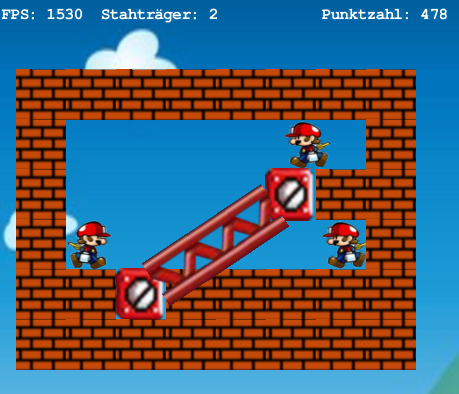
\includegraphics[scale=1]{\basepath/\shortGameTitle/beams.png}
\caption{Der Mario ganz links sowie der obere Mario k"onnen den Stahltr"ager hoch- und runterlaufen. Der Mario unten rechts jedoch wird von ihm eingeschlossen.}
\label{beams}
\end{center}
\end{figure}